
\section{Hardware and operating system configuration}

The sections below may be useful in setting up your cluster and operating system (including the user account that will be running DiFX).

\subsection{Cluster configuration} \label{sec:cluster}

For production correlation, it is suggested that a dedicated user account be created; for the rest of this document it will be assumed to be ``difx''.
This account should have few or no other uses in order to ensure that the environment is not disturbed.
The user account must exist on all nodes in the cluster and ssh should be configured so that no password is required when logging into one node on the cluster from another.
This user account must also exist on the Mark5 units that are used for playback.
It is recommended that all computers in the cluster, including the Mark5s, run the same version of Linux to avoid library compatibility issues.

All of the nodes in the cluster, including the Mark5s, should be interconnected by a fast network and have NFS access to the directories from which correlation is to proceed.
Complicated network topologies, such as having more than one cluster node attached to more than one network, can lead to unpredictable results as OpenMPI (the suggested MPI library to use with {\tt mpifxcorr}) is network aggressive and will use any means possible to enhance performance, even if such antics are counterproductive.
If your network topology is not simple be aware of any network-related issues and keep in mind that you might need to explicitly specify which network interfaces to use.

One node should be deemed the ``head node''.
In general this node should have lots of hard disk space which is cross mounted to all the others and could serve as the network gateway to the remainder of the cluster.
It is convenient, but not necessary, to locate all of the software and correlation directories physically on this node to improve the interchangeability of the other nodes.
This node can participate in the actual correlation, either as the manager node, a processing node or both.
By default, the head node will always be the manager node.


\subsection{Environment variables} \label{sec:env}

In addition to environment variables needed at build-time (\S\ref{sec:install}), some others are needed at run time.
These are:
\begin{enumerate}
\item {\tt CALC\_SERVER} contains the name of the computer running calcServer (\S\ref{sec:calcserver}).
This is accessed only by program {\tt calcif}.
\item {\tt DIFX\_ARCHIVE\_ROOT} points to the base directory of the archive staging area.
\item {\tt DIFX\_ARCHIVE\_USERNAME} specifies the username of the archiving process (NRAO use only).
\item {\tt DIFX\_CALC\_PROGRAM} specifies the command used to evaluate the delay model.  By default this is currently {\tt calcif2}, however it is expected this will change to {\tt difxcalc} in the DiFX 2.6 release series.
\item {\tt DIFX\_GROUP\_ID} the Unix group to use.  If set, umask is changed to 002 and all new files/directories become group writable.
\item {\tt DIFX\_HEAD\_NODE} contains the name of the cluster head node.
\item {\tt DIFX\_MACHINES} points to a file containing a list of cluster members and their capabilities.
See \S\ref{sec:difxmachines}
\item {\tt DIFX\_MESSAGE\_GROUP} (optional) specifies, with {\tt DIFX\_MESSAGE\_PORT}, the multicast group and port to be used for GUI and monitoring.
\item {\tt DIFX\_MESSAGE\_PORT} (optional, {\em see above})
\item {\tt DIFX\_QUEUE\_BASE} points to the base of the correlator staging area for jobs to be run.
\item {\tt DIFX\_VERSION} (optional, but recommended) the version of difx being used, e.g., {\tt DIFX-2.2} .
\item {\tt EVLAMPTS\_DB} contains the connection information for the Postgress E
VLA monitor point database (NRAO only, needed only if VLA is included in array).
\item {\tt GAIN\_CURVE\_PATH} (optional) points to a directory that contains keyin format files containing gain curves.
This is used only by {\tt difx2fits}.
If not set, {\tt difx2fits} will not create gain curve tables.
This directory must be readable by the difx user.
Every file in this directory will be read, assuming it is a keyin format gain curve, so nothing else should be stored here.
This directory needs to be created by hand if it does not exist.
\item {\tt JOB\_ROOT} points to the base directory that is to contain copies of job scripts of projects to correlate.
This directory must be visible by all nodes on the cluster.
\item {\tt DIFX\_LOG\_DIR} points to the directory where logs shall be written.
\item {\tt MARK5\_DIR\_PATH} points to a directory that is used to cache the contents of Mark5 modules.
This directory must be readable and writable by the user running mpifxcorr.
This directory needs to be created by hand if it does not exist.  
It will get populated automatically.
If there are problems with playback of a module, the files in this directory can sometimes be useful.
\item {\tt MARK6\_ROOT} points to the mountpoints for Mark6 files.
The default is {\tt /mnt/disks/*/*/data}.
\item {\tt PGPLOT\_FONT} points to a font file for PGPLOT.
The font file is usually called {\tt grfont.dat} .
\item {\tt TCAL\_PATH} points to a directory containing $T_{\rm cal}$ values for receivers.
\item {\tt TESTS} points to a path containing test data projects.
\item {\tt VLBA\_DB} contains the connection information for the Oracle legacy VLBA database (NRAO only).
\item {\tt VLBAMPTS\_DB} contains the connection information for the Postgress EVLA-style VLBA monitor point database (NRAO only).
\end{enumerate}
Like the environment variables described in \S\ref{sec:install}, these should all be set in shell initialization files and should be set whether the shell is used interactively or not.
For the {\tt difx} user account at NRAO, these are set in a file called {\tt setup\_difx} which is run upon login (see \S\ref{sec:versions}).
Note that this file needs to be run whether the login is interactive or not; please consult the documentation for your shell if you have problems.
To test if this file is being run in non-interactive sessions, try the following: {\tt ssh} {\em computername} {\tt env | grep DIFX} and make sure you see the environment variables you expect to.


\subsection{Directory structure and versioning} \label{sec:versions}

The directory structure of the NRAO deployment of DiFX is outlined in Fig.~\ref{fig:dirtree}.
The aim is to cleanly programs, libraries, and other version-specific files from data in a way that switching from one version (e.g., 1.5) to another (e.g., the development version) is simple, accountable, and complete, in order to assure that a self-consistent set of software is used for an entire project.
Each DiFX version has its own root directory, such as {\tt /home/swc/DiFX-1.5} .
All files associated with this version are under this directory.
No data or files associated with any other DiFX version shall be placed within.

Setting up a particular version is quite simple.
Assuming the {\tt bash} shell:

{\tt . /home/swc/DiFX-1.5/setup\_difx}

This script contains, among other lines, the following:

\begin{verbatim}
export DIFX_PREFIX=/home/swc/NRAO-DiFX-trunk
export DIFX_BASE=/home/swc/difx
export DIFX_ARCHIVE_ROOT=/home/ngas_staging/difx
export JOB_ROOT=${DIFX_BASE}/projects
export TESTS=${DIFX_BASE}/tests
export MARK5_DIR_PATH=${DIFX_BASE}/directories
export CALC_SERVER=swc000
export GAIN_CURVE_PATH=${DIFX_BASE}/gaincurves
export DIFX_MACHINES=${DIFX_BASE}/machines.difx
export DIFX_QUEUE_BASE=${DIFX_BASE}/queue
export DIFX_HEAD_NODE=swc000
export DIFX_VERSION=DIFX-1.5
export DIFX_GROUP_ID=vlba_difx
export DIFX_MESSAGE_GROUP=224.2.2.1
export DIFX_MESSAGE_PORT=50200
export IPPROOT=/home/swc/difx/intel/ipp/6.0.2.076/ia32
export PATH=${DIFX_PREFIX}/bin:${ORACLE_HOME}/bin:/users/difx/bin:/bin:/usr/bin
export LD_LIBRARY_PATH=${DIFX_PREFIX}/lib:${IPPROOT}/sharedlib:${ORACLE_HOME}/lib
echo "DIFX version 1.5 is selected"
\end{verbatim}

The ``difx'' account is set up to execute this script upon login.
Note that the settings here are useful for both compilation of the various DiFX components as well as using them.
Each installed version of DiFX will have its own setup file like this.
Selecting which version is to be used is a simple as running the correct setup file.
To change to the development version:

{\tt . /home/swc/DiFX-trunk/setup\_difx}

\begin{figure}[h]
\begin{center}
\resizebox{4.9in}{!}{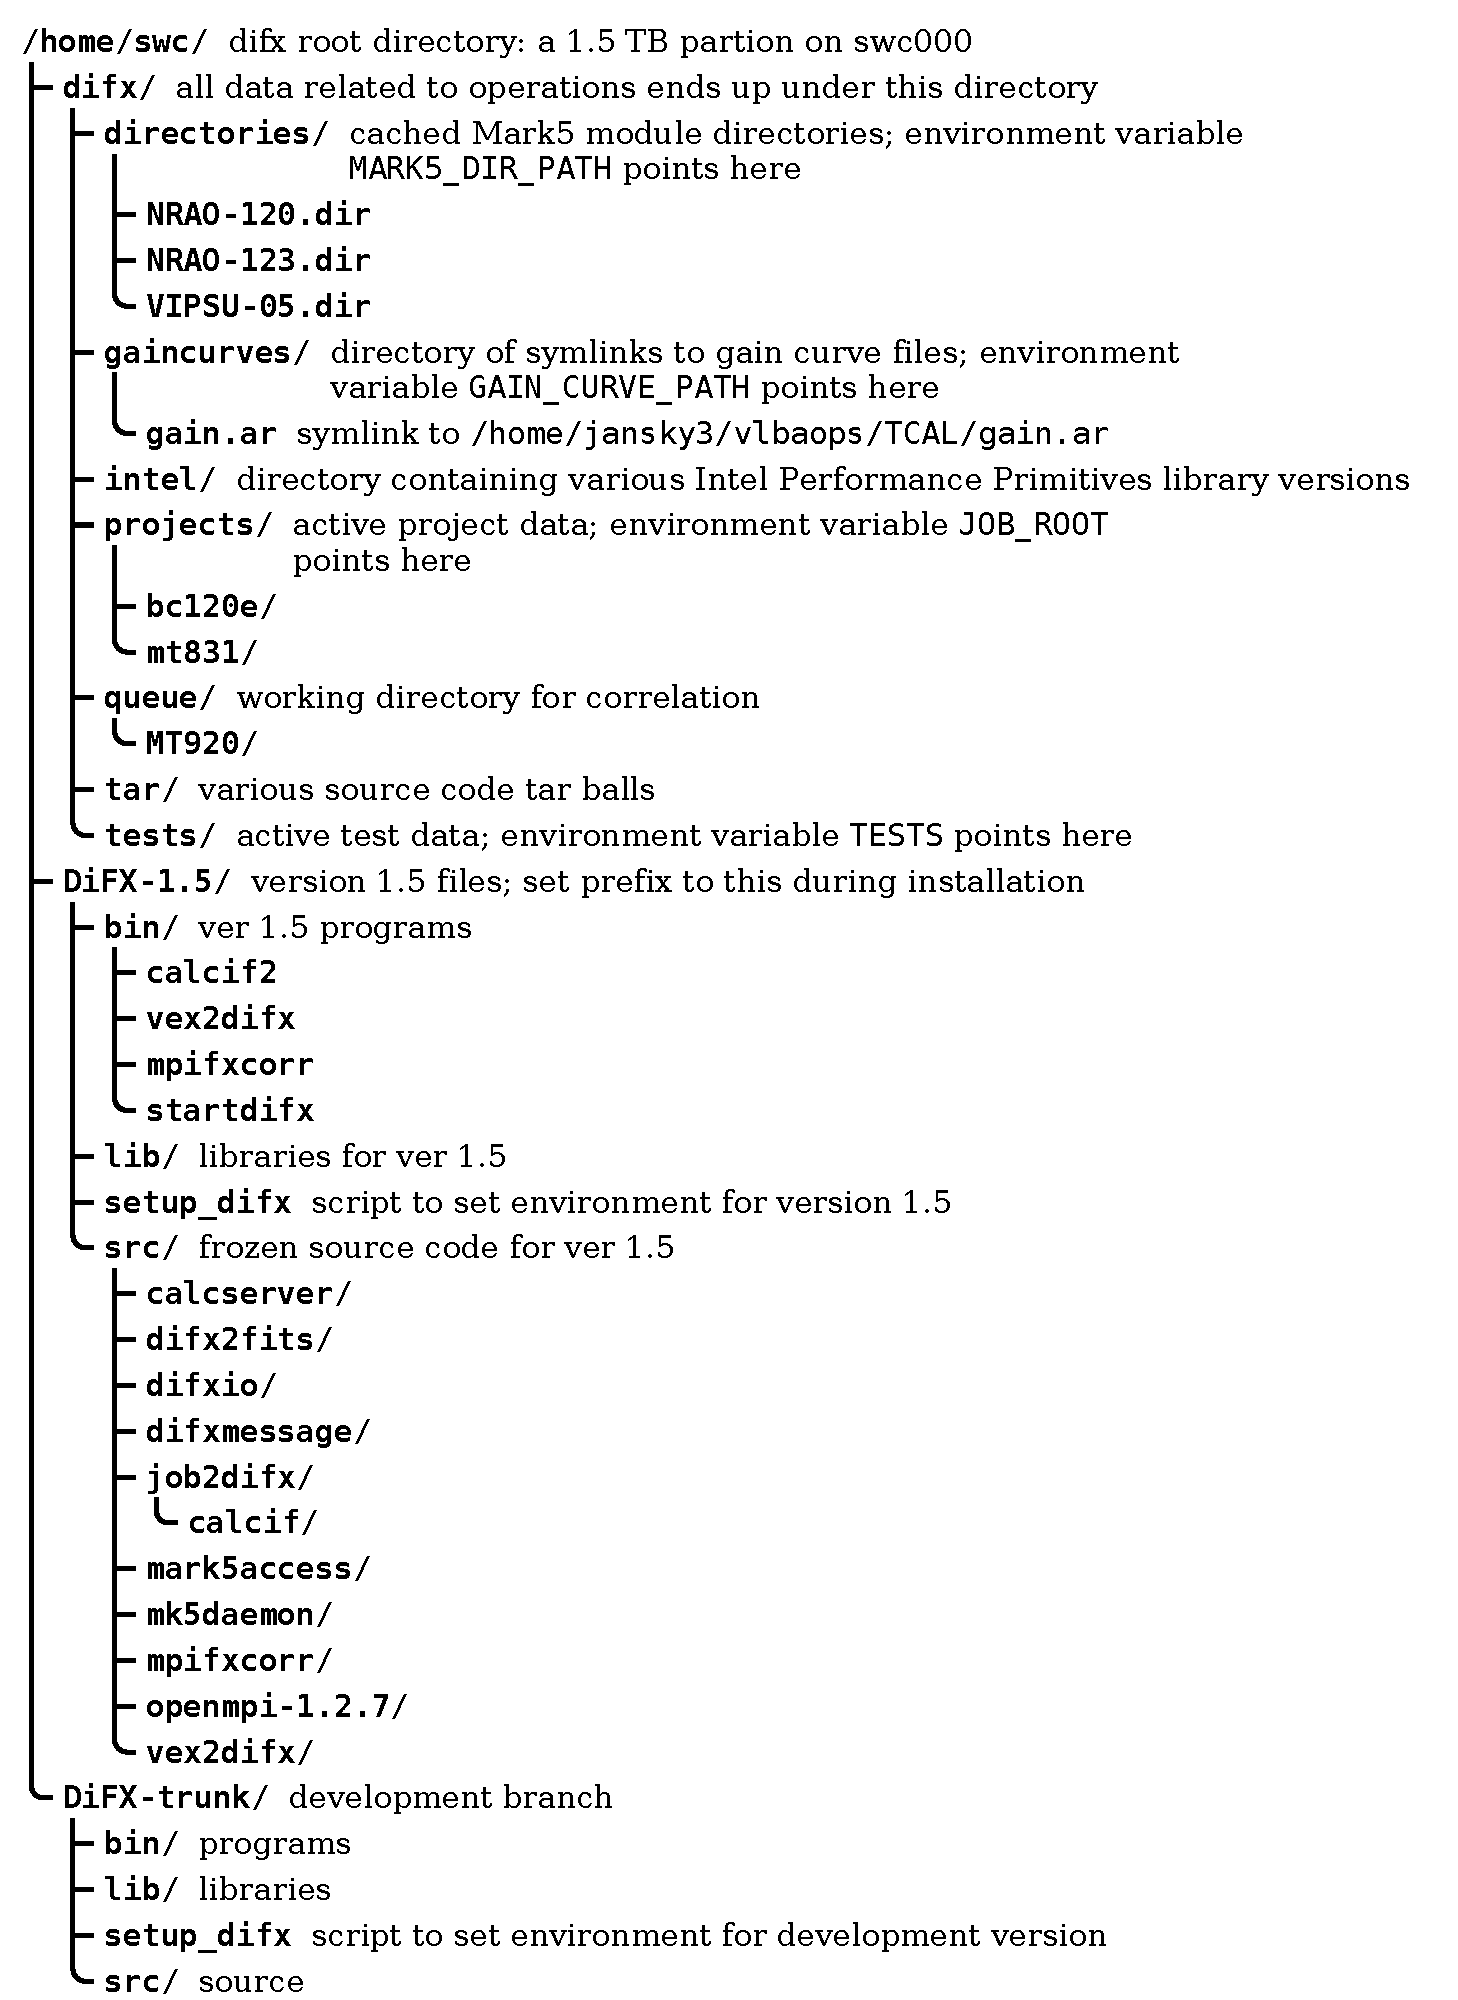
\includegraphics{tree}}
\caption[dirtree]{
{\em The directory structure of the VLBA software correlator.}  
This figure showing the organization of the DiFX directory structure is not comprehensive, but is hopefully complete enough to illustrate the general layout.
For example, only the major top level subdirectories of {\tt DiFX-trunk} are shown.
Entries ending in `/' are themselves directories.
\label{fig:dirtree}
}
\end{center}
\end{figure}

It is highly recommended that one set the {\tt DIFX\_VERSION} environment variable and make sure that for each installed version of DiFX this is set differently.
It may also be desirable to customize this for your correlator.
For example, one may set it to {\tt USNO-DIFX-1.5} .
This string will be stored in intermediate files and the output FITS files and will be able to identify more exactly where the data were correlated.
